

\section{Multiple Regression in R}

To illustrate multiple regression in R we'll use a built in dataset called |trees|. |trees| consists of measurements of the girth, height, and volume of 31 black cherry trees (|?trees| for more info). We'll start with some summary tables and diagnostic plots to familiarize ourselves with the data:
%
\begin{R}
> names(trees)
[1] "Girth"  "Height" "Volume"
> dim(trees)
[1] 31  3
> summary(trees)
     Girth           Height       Volume
 Min.   : 8.30   Min.   :63   Min.   :10.20
 1st Qu.:11.05   1st Qu.:72   1st Qu.:19.40
 Median :12.90   Median :76   Median :24.20
 Mean   :13.25   Mean   :76   Mean   :30.17
 3rd Qu.:15.25   3rd Qu.:80   3rd Qu.:37.30
 Max.   :20.60   Max.   :87   Max.   :77.00

# we'll use the chart.Correlation fxn that we introduced last week 
> library(PerformanceAnalytics)  
> chart.Correlation(trees)
\end{R}
%
As one might expect, the scatterplot matrix shows that all the variables are positively correlated, and girth and volume have a  particularly strong correlation.

Let's assume we're lumberjacks, but our permit only allows us to harvest a fixed number of trees.  We get paid by the total volume of wood we harvest, so we're interested in predicting a tree's volume (hard to measure directly) as a function of its girth and height (relatively easy to measure), so we can pick the best trees to harvest.  We'll therefore calculate a multiple regression of volume on height and width. Let's start by taking a look at the 3D scatter of the data using the plot3d function from the |rgl| package.
%
\begin{R}
> library(rgl)
> plot3d(trees, col='red', size=1, type='s') # use your mouse to rotate the plot
\end{R}
%
From the 3D scatter plot it looks like we ought to be able to find a plane through the data that fits the scatter fairly well. Let's use the |lm()| function to calculate the multiple regression:
%
\begin{R}
> l <- lm(Volume ~ Girth + Height, data=trees)
\end{R}
%
To visualize the multiple regression, let's use the |scatterplot3d| package to draw the 3D scatter of plots and the plane that corresponds to the regression model:
%
\begin{R}
> library(scatterplot3d)  # install this package first if needed
> p <- scatterplot3d(trees,angle=55,type='h')
> title('Tree Volume as\na function of Girth and Height')
> p$plane3d(l, col='orangered')
> dev.copy(pdf, 'trees-regrfit.pdf')  # copy plot to a pdf file
> dev.off()  # write the file
\end{R}
%
Notice the use of |dev.copy()| and |dev.off()| to save the plot from the console.  The output this generates should look similar to Fig.~\ref{fig:treesregr}.
%
\begin{figure}[htbp]
\centering
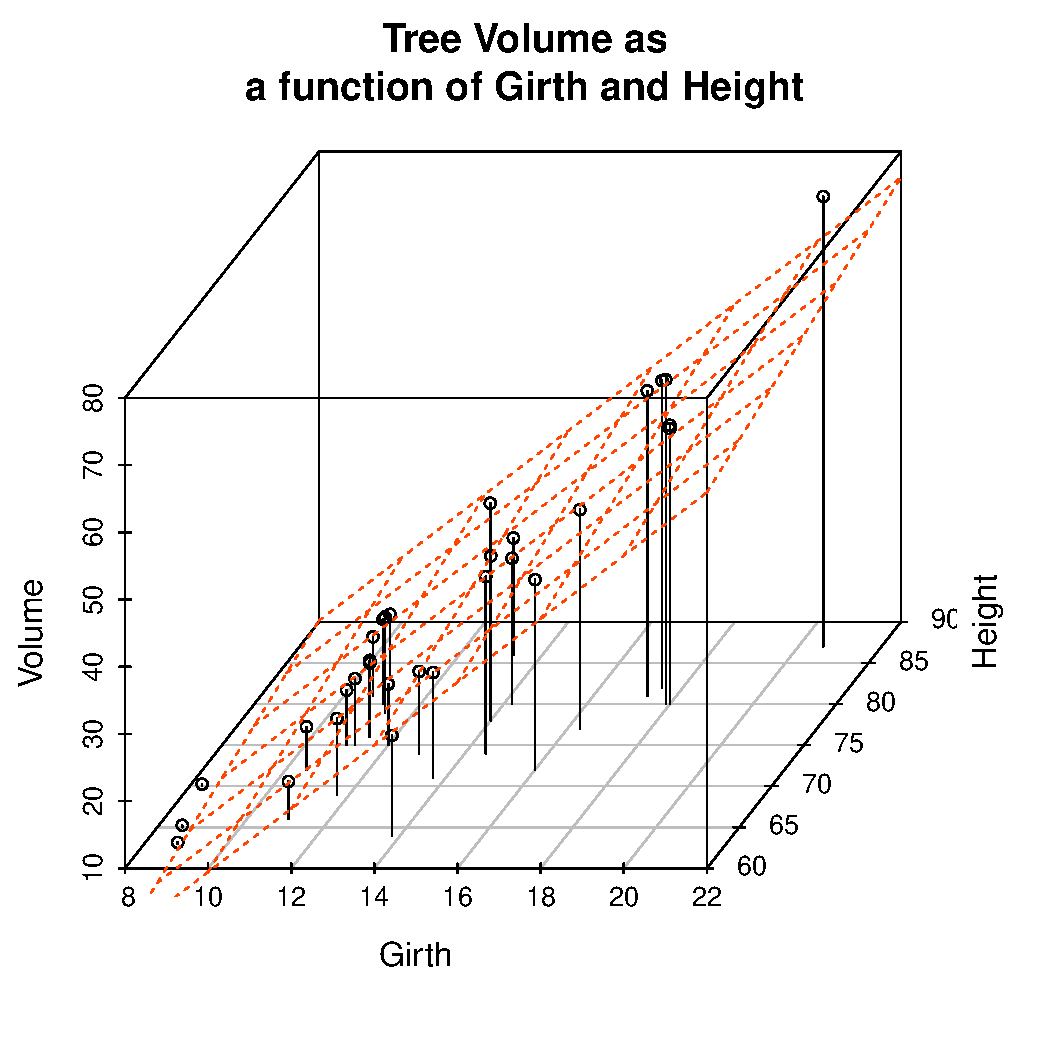
\includegraphics[width=0.5\columnwidth]{./figures/hands-on4/trees-regrfit.pdf}
\caption{Multiple regression plot of cherry tree volume on girth and height, generated using the \texttt{scatterplot3d} library\label{fig:treesregr}}
\end{figure}

From the figure it looks like the regression model fits pretty well, as we anticipated  from the pairwise relationships.  Let's use the |summary()| function to obtain details of the model:
\begin{R}
> summary(l)

Call:
lm(formula = Volume ~ Girth + Height, data = trees)

Residuals:
    Min      1Q  Median      3Q     Max
-6.4065 -2.6493 -0.2876  2.2003  8.4847

Coefficients:
            Estimate Std. Error t value Pr(>|t|)
(Intercept) -57.9877     8.6382  -6.713 2.75e-07 ***
Girth         4.7082     0.2643  17.816  < 2e-16 ***
Height        0.3393     0.1302   2.607   0.0145 *
---
Signif. codes:  0 ‘***’ 0.001 ‘**’ 0.01 ‘*’ 0.05 ‘.’ 0.1 ‘ ’ 1

Residual standard error: 3.882 on 28 degrees of freedom
Multiple R-squared: 0.948,  Adjusted R-squared: 0.9442
F-statistic:   255 on 2 and 28 DF,  p-value: < 2.2e-16
\end{R}
%
The regression equation is: $\hat{y} = 4.71x_1 + 0.34x_2$, where $y$ is Volume, and $x_1$ and $x_2$ are Girth and Height respectively. Since they're on different scales the coefficients for Girth and Height aren't directly comparable. Both coefficients are significant at the $p<0.05$ level, but note that Girth is the much stronger predictor. In fact the addition of height explains only a minor additional fraction of variation in tree volume, so from the lumberjack's perspective the additional trouble of measuring height probably isn't worth it.

\subsection{Exploring the Vector Geometry of a Regression Model}

The object returned by the |lm()| function hold lots of useful information:
%
\begin{R}
> names(l)
 [1] "coefficients"  "residuals"     "effects"       
     "rank"          "fitted.values" "assign"
 [7] "qr"            "df.residual"   "xlevels" 
     "call"          "terms"         "model"
\end{R}
%
The |fitted.values| correspond to the predicted values of the outcome variable ($\hat{y}$). Let's use our knowledge of vector geometry to further explore the relationship between the predicted Volume and the predictor variables.  By definition the vector representing the predicted values lies in the plane defined by Height and Girth, so let's do some simple calculations to understand their length and angular relationships:
%
\begin{R}
# proportional to length of vectors
> sd(l$fitted.values)
[1] 16.00434
> sd(trees$Height)
[1] 6.371813
> sd(trees$Girth)
[1] 3.138139

# cosines of angles btw vectors
> cor(trees$Height, trees$Girth)
[1] 0.5192801
> cor(trees$Height, l$fitted.values)
[1] 0.6144545
> cor(trees$Girth, l$fitted.values)
[1] 0.9933158

# angles btw vectors in degrees
> acos(cor(trees$Height, l$fitted.values)) * (180/pi)
[1] 52.08771
> acos(cor(trees$Girth, l$fitted.values)) * (180/pi)
[1] 6.628322
> acos(cor(trees$Girth, trees$Height)) * (180/pi)
[1] 58.71603
\end{R}
%

\begin{tcolorbox}[title=In class assignment]
Using the calculations above you should now be able to sketch out by hand, a diagram depicting the vector relationships between Height, Girth, and the predicted Volume .  Once you've finished with your sketch, discuss it with your fellow classmates.  Did you get similar answers? If not, discuss it and try to come up with an agreed upon representation.
\end{tcolorbox}

\subsection{Exploring the Residuals from the Model Fit}

Now let's look at the residuals from the regression. The residuals represent the `unexplained' variance:
\begin{R}
> plot(trees$Volume,l$residuals, xlab='Volume',ylab='Regression Residuals')
> abline(h=0, lty='dashed', col='red')
\end{R}
%
Ideally the residuals should be evenly scattered around zero, with no trends as we go from high to low values of the dependent variable.  As you can see in Fig.~\ref{fig:trees-resid} it looks like that the residuals on the left tend to be below zero, while those on the far right of the plot are consistently above zero, suggesting that there may be a non-linear aspect of the relationship that our model isn't capturing.
%
\begin{figure}[htbp]
\centering
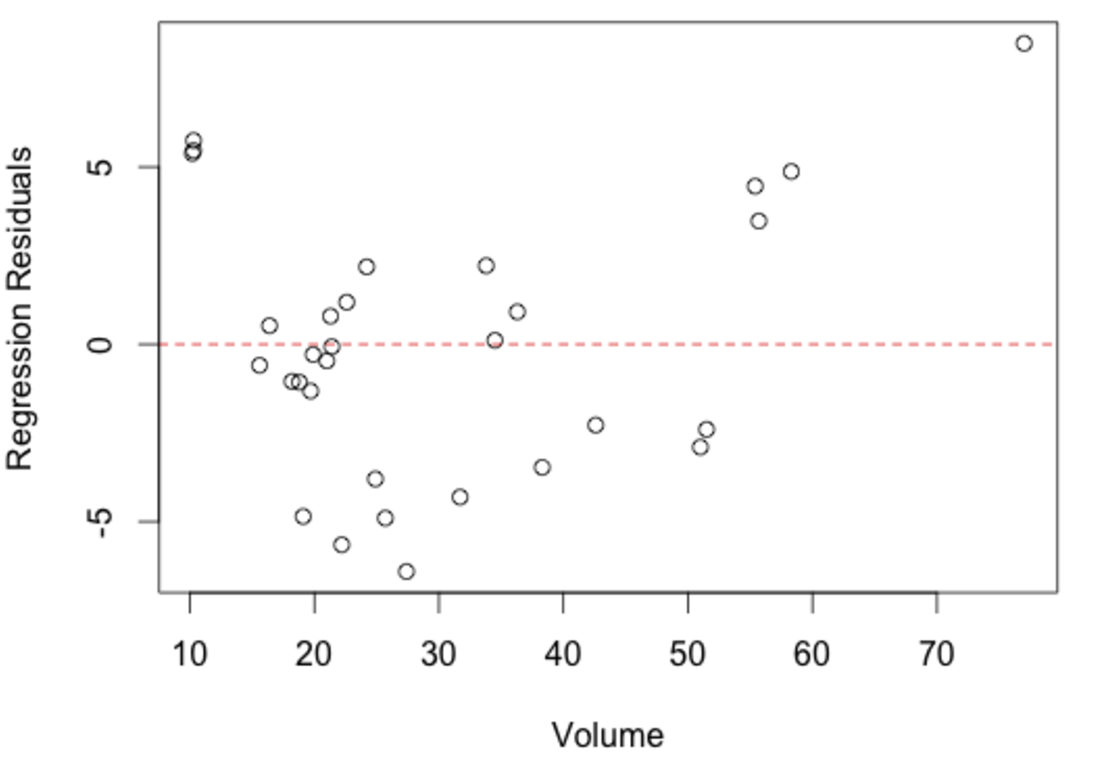
\includegraphics[height=1.5in]{./figures/hands-on4/trees-residuals.pdf}
\caption{Residual plot based on the multiple regression plot of cherry tree volume on girth and height,\label{fig:trees-resid}}
\end{figure}

Let's think about the relationships we're actually modeling for a few minutes.  For the sake of simplicity let's consider the trunk of a tree to be a cylinder.  How do the dimensions of this cylinder relate to its volume? You can look up the formula for the volume of a cylinder, but the key thing you'll want to note is that volume of the cylinder should be proportional to a characteristic length of the cylinder cubed ($V \propto \mathrm{L}^3$). This suggests that if we want to fit a linear model we should relate Girth to $\sqrt[3]{\mathrm{Volume}}$. Let's explore this a little. Since our initial multiple regression suggested that height had relatively little predictive power, we'll simplify our model down to a single predictor:
%
\begin{R}
> cuberoot.V <- trees$Volume^0.33
> cor(trees$Volume, trees$Girth)
[1] 0.9671194
> cor(cuberoot.V, trees$Girth)
[1] 0.9777078
> l.orig <- lm(trees$Volume~ trees$Girth)
> l.transf <- lm(cuberoot.V ~ trees$Girth)
> summary(l.orig)

Call:
lm(formula = trees$Volume ~ trees$Girth)

Residuals:
   Min     1Q Median     3Q    Max
-8.065 -3.107  0.152  3.495  9.587

Coefficients:
            Estimate Std. Error t value Pr(>|t|)
(Intercept) -36.9435     3.3651  -10.98 7.62e-12 ***
trees$Girth   5.0659     0.2474   20.48  < 2e-16 ***
---
Signif. codes:  0 ‘***’ 0.001 ‘**’ 0.01 ‘*’ 0.05 ‘.’ 0.1 ‘ ’ 1

Residual standard error: 4.252 on 29 degrees of freedom
Multiple R-squared: 0.9353, Adjusted R-squared: 0.9331
F-statistic: 419.4 on 1 and 29 DF,  p-value: < 2.2e-16

> summary(l.transf)

Call:
lm(formula = cuberoot.V ~ trees$Girth)

Residuals:
     Min       1Q   Median       3Q      Max
-0.18919 -0.09775 -0.01488  0.07855  0.26427

Coefficients:
            Estimate Std. Error t value Pr(>|t|)
(Intercept)  0.82543    0.08856   9.321 3.18e-10 ***
trees$Girth  0.16324    0.00651  25.076  < 2e-16 ***
---
Signif. codes:  0 ‘***’ 0.001 ‘**’ 0.01 ‘*’ 0.05 ‘.’ 0.1 ‘ ’ 1

Residual standard error: 0.1119 on 29 degrees of freedom
Multiple R-squared: 0.9559, Adjusted R-squared: 0.9544
F-statistic: 628.8 on 1 and 29 DF,  p-value: < 2.2e-16
\end{R}
%
Comparing the summary tables, we see indeed that using the cube root of Volume improves the fit of our model some. Let's examine the residuals.
%
\begin{R}
> layout(c(1,2), widths=c(3,3), heights=c(2,2))
> plot(trees$Volume, l.orig$residuals, xlab='Volume', ylab="Residuals")
> abline(h = 0, col='red', lty='dashed')
> plot(cuberoot.V, l.transf$residuals, 
        xlab='Volume^0.33', ylab='Residuals')

> abline(h = 0, col='red', lty='dashed')
> dev.copy(pdf, 'compare-residuals.pdf')
> dev.off()
> layout(c(1,1))   # reset the layout
\end{R}
%
\begin{figure}[htbp]
\centering
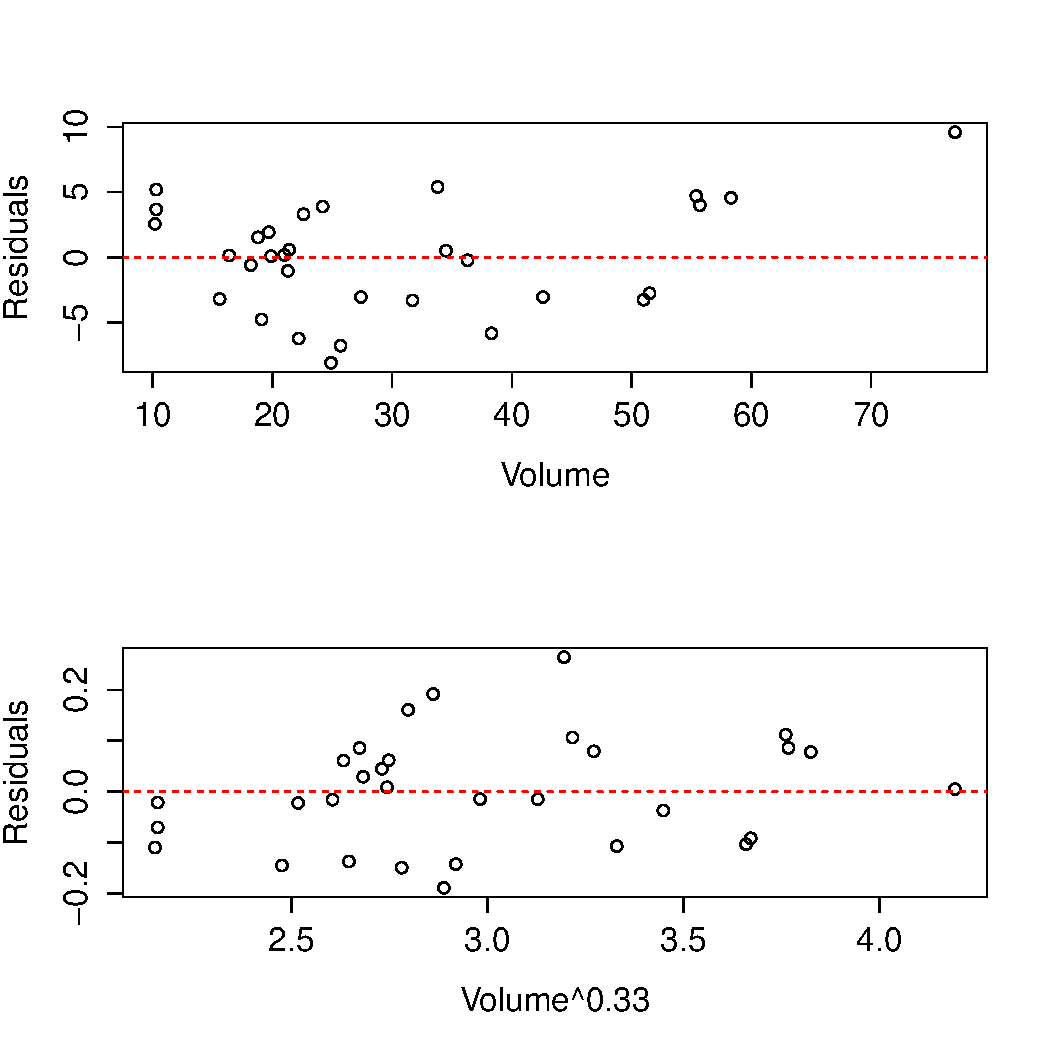
\includegraphics[height=2in]{./figures/hands-on4/compare-residuals.pdf}
\caption{Residual plot based on the bivariate regression of tree volume on girth, or $\sqrt[3]{V}$ on girth \label{fig:compare-resid}}
\end{figure}
%
As we can see the transformation we applied to the data did seem to make our residuals more uniform across the range of observations. Note the use of the |layout()| function to put multiple plots in the same figure.

\subsection{Fitting a curvilinear model using lm()}

Above we transformed the volume data in order to fit a straight line relationship between $\sqrt[3]{V}$  and Girth. However, we could just as easily have applied a cubic regression to the original variables as shown below (remember this is still linear  in the coefficients):

\begin{R}
> lm.3 <- lm(Volume ~ I(Girth^3), data=trees)
> summary(lm.3)

Call:
lm(formula = Volume ~ I(Girth^3), data = trees)

Residuals:
   Min     1Q Median     3Q    Max
-4.526 -3.036  0.215  2.419  8.291

Coefficients:
             Estimate Std. Error t value Pr(>|t|)
(Intercept) 8.0426960  1.0426698   7.714 1.66e-08 ***
I(Girth^3)  0.0081365  0.0003118  26.098  < 2e-16 ***
---
Signif. codes:  0 ‘***’ 0.001 ‘**’ 0.01 ‘*’ 0.05 ‘.’ 0.1 ‘ ’ 1

Residual standard error: 3.379 on 29 degrees of freedom
Multiple R-squared: 0.9592, Adjusted R-squared: 0.9578
F-statistic: 681.1 on 1 and 29 DF,  p-value: < 2.2e-16

> lm.3$coefficients
(Intercept)  I(Girth^3)
8.042696007 0.008136533
> a0 = lm.3$coefficients[[1]]
> B1 = lm.3$coefficients[[2]]
> x <- seq(8,25,0.25) # range of values to evaluate model over
> fit <- a0 + B1*x^3
> plot(Volume ~ Girth, data=trees)
> lines(x,fit,col='red')
> figtext <- paste(c("Volume = ", round(a0,2), "+", round(B1,4), "*Girth^3"), collapse='')
> text(12, 60, figtext)
\end{R}
%
\begin{figure}[htbp]
\centering
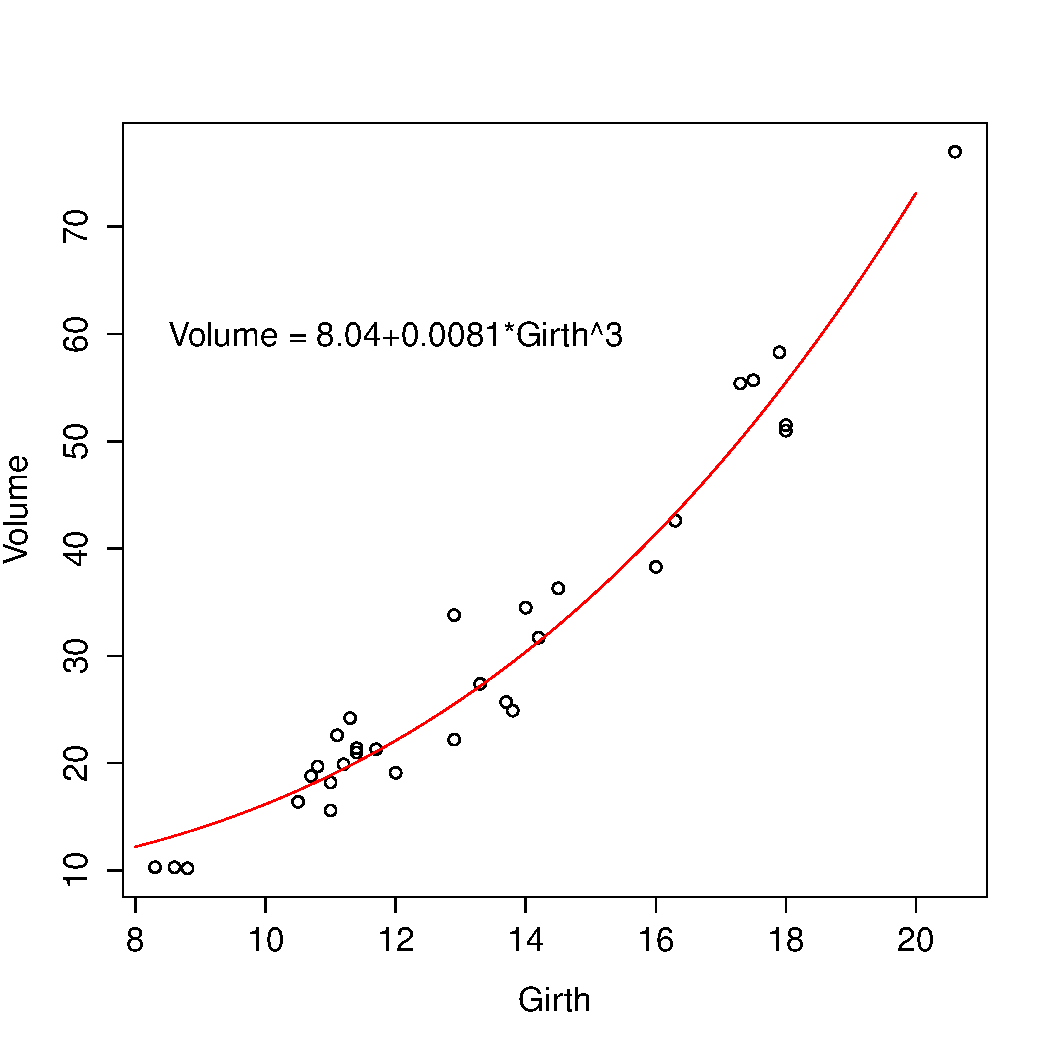
\includegraphics[height=2in]{./figures/hands-on4/cubic-regr.pdf}
\caption{Cubic regression of tree volume on girth \label{fig:cubic-regr}}
\end{figure}
%
The |I()| function used above requires a little explanation.  Normally, the R formula syntax (see |?formula|) treats the carat symbol, |'^'|, as short-hand for factor crossing to the specified degree.  For example, the formula |(a+b+c)^2| would be interpretted as the model with main effects and all second order interaction terms, i.e. |a + b + c + a:b + a:c + b:c| where the colons indicate interactions.  The |I()| function `protects' the object in it's argument; in this case telling the regression function to treat this as Girth raised to the third power as opposed to trying to construct interaction terms for Girth.


\medskip
\begin{assignment}
Write a function, |mult.regr(X,y)| that calculates the multiple regression of $y$ on multiple predictors, $x_1, x_2, \ldots x_k$ \emph{using matrix operations}. Your function should take two arguments, |X| and |y|, where |X| is a matrix representing the predictor variables and |y| is a vector for the outcome variable.  Your function should return a list containg the vector of regression coeffients, $B$, the coefficient of determination ($R^2$), and a vector, $\hat{y}$, representing the fitted values.  Refer to the slides from lecture 4 (and possibly lecture 2 if you need a refresher) to review the matrix  solution to the regression problem.
\end{assignment}


\section{Exploring the impact of nearly collinear predictors on regression}

In lecture we discussed the problems that can arise in regression when your predictor variables are nearly collinear. In this section we'll illustrate some of these issues.

Consider again the |trees| data set.  Recall that two of the variables -- Girth and Volume -- are highly correlated and thus nearly collinear.
%
\begin{R}
> cor(trees)
           Girth    Height    Volume
Girth  1.0000000 0.5192801 0.9671194
Height 0.5192801 1.0000000 0.5982497
Volume 0.9671194 0.5982497 1.0000000
\end{R}
%
Let's explore what happens when we treat Height as the dependent variable, and Girth and Volume as the predictor variables.
%
\begin{R}
> lm.H <- lm(Height ~ Girth + Volume, data = trees)
> summary(lm.H)

Call:
lm(formula = Height ~ Girth + Volume, data = trees)

Residuals:
    Min      1Q  Median      3Q     Max 
-9.7855 -3.3649  0.5683  2.3747 11.6910 

Coefficients:
            Estimate Std. Error t value Pr(>|t|)    
(Intercept)  83.2958     9.0866   9.167 6.33e-10 ***
Girth        -1.8615     1.1567  -1.609   0.1188    
Volume        0.5756     0.2208   2.607   0.0145 *  
---
Signif. codes:  0 ‘***’ 0.001 ‘**’ 0.01 ‘*’ 0.05 ‘.’ 0.1 ‘ ’ 1

Residual standard error: 5.056 on 28 degrees of freedom
Multiple R-squared:  0.4123,    Adjusted R-squared:  0.3703 
F-statistic:  9.82 on 2 and 28 DF,  p-value: 0.0005868
\end{R}
%
We can, of course, fit the linear model despite the collinearity, and we find that the model does have some predictive power, with $R^2 = 0.41$, and with Volume being the more significant predictor.

Now, let's created a slightly different version of the trees data set by add some noise to the three variables.   Our goal here is to simulate a data set we might have created had we measured a slightly different set of trees during our sampling. We'll use the |jitter| function to add uniform noise to the data set.
%
\begin{R}
> jitter.Girth <- jitter(trees$Girth, amount= 0.25 * sd(trees$Girth))
> jitter.Height <- jitter(trees$Height, amount= 0.25 * sd(trees$Height))
> jitter.Volume <- jitter(trees$Volume, amount= 0.25 * sd(trees$Volume))
> jitter.trees <- data.frame(Girth = jitter.Girth, 
                        Height = jitter.Height, 
                        Volume = jitter.Volume)
\end{R}
%
Here we added uniform noise proportional to the one-quarter the standard deviation of each variable.  Let's take a moment to convince ourselves that our new data set, |jitter.trees|, is not too different from the |trees| data set from which it was derived.
%
\begin{R}
# compare this to summary(trees)
# You will get slightly different answers because jitter adds random noise

> summary(jitter.trees)
     Girth            Height          Volume     
 Min.   : 7.913   Min.   :62.31   Min.   :10.75  
 1st Qu.:10.971   1st Qu.:72.37   1st Qu.:18.99  
 Median :12.606   Median :76.54   Median :22.38  
 Mean   :13.170   Mean   :75.84   Mean   :29.77  
 3rd Qu.:15.183   3rd Qu.:80.63   3rd Qu.:37.71  
 Max.   :20.722   Max.   :85.91   Max.   :77.69  

# correlations among jittered variables are
# similar to those of the original variables

> cor(jitter.trees)
           Girth    Height    Volume
Girth  1.0000000 0.4924240 0.9433214
Height 0.4924240 1.0000000 0.5531763
Volume 0.9433214 0.5531763 1.0000000    

## jittered variables are highly correlatd with original variables

> cor(trees$Height, jitter.trees$Height)
[1] 0.9861006
> cor(trees$Girth, jitter.trees$Girth)
[1] 0.9928097
> cor(trees$Volume, jitter.trees$Volume)
[1] 0.9883385

> plot(trees$Height, jitter.trees$Height)
> plot(trees$Girth, jitter.trees$Girth)
> plot(trees$Volume, jitter.trees$Volume)
\end{R}

Now that we've convinced ourselves that our jittered data set is a decent approximation to our original data set, let's re-calculate the linear regression, and compare the coefficients of the jittered model to the original model:
%
\begin{R}
> lm.H.jitter <- lm(Height ~ Girth + Volume, data = jitter.trees)
> coefficients(lm.H.jitter)
(Intercept)       Girth      Volume 
 73.3492169  -0.5437115   0.3241854 
> coefficients(lm.H)
(Intercept)       Girth      Volume 
 83.2957705  -1.8615109   0.5755946 
\end{R}
%
We see that the coefficients of the linear model have changed quite a bit between the original data and the jittered data.  Our model is unstable to relatively modest changes to the data!

Let's  draw some plots to illustrate how different the models fit to the original and jittered data are:
%
\begin{R}
# draw 3d scatter plots with small points so as not to obscure regression planes
> p <- scatterplot3d(x=trees$Girth, y=trees$Volume, z=trees$Height, 
                      angle=15, type='p', pch='.')

# original model
> p$plane3d(lm.H, col='orangered')

# jittered model
> p$plane3d(lm.H.jitter, col='blue')
\end{R}
%
The figure you generated should look something like Fig.~\ref{fig:jittercompare}.
%
\begin{figure}[htbp]
\centering
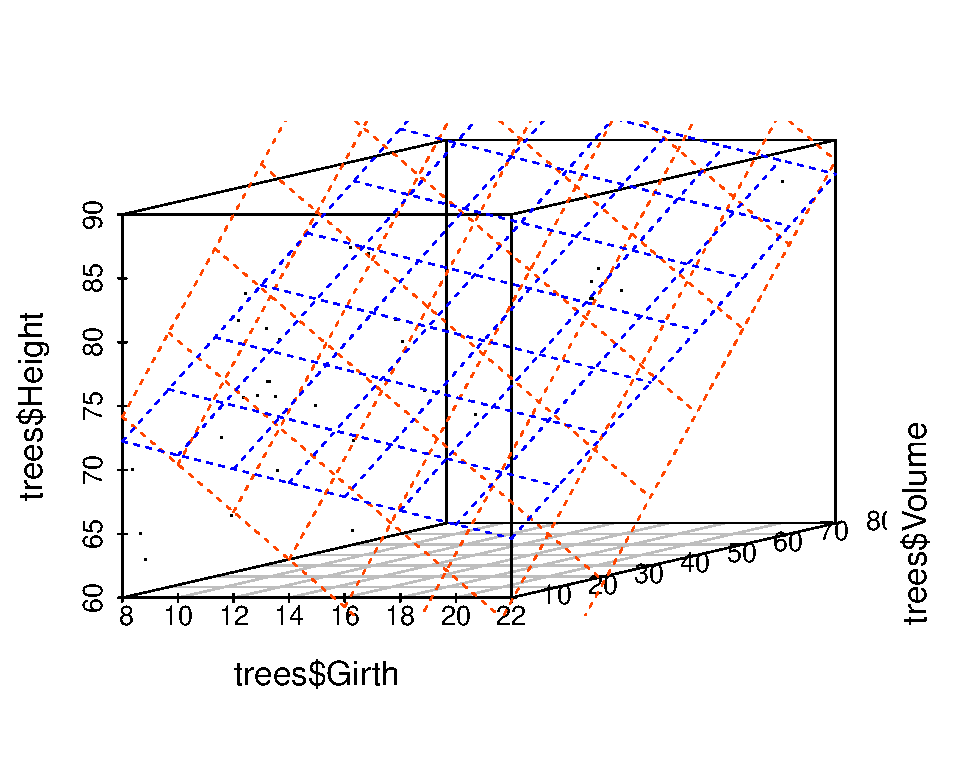
\includegraphics[width=0.5\columnwidth]{./figures/hands-on4/trees-jitterfit-height.pdf}
\caption{Multiple regression plot of cherry tree height on girth and volume, for the original data (red) and the jittered data (blue).\label{fig:jittercompare}}
\end{figure}



Let's do the same comparison for the multiple regression of Volume on Height and Girth.  In this case the predictor variables are \emph{not} nearly collinear.
%
\begin{R}
> lm.V <- lm(Volume ~ Girth + Height, data = trees)
> lm.V.jitter <- lm(Volume ~ Girth + Height, data = jitter.trees)
> coefficients(lm.V)
(Intercept)       Girth      Height 
-57.9876589   4.7081605   0.3392512 
> coefficients(lm.V.jitter)
(Intercept)       Girth      Height 
-51.2670818   4.4798268   0.2906203 
\end{R}
%
For this model, we see that the coefficients have changed only a small amount.  The underlying data, |jitter.trees|, is the same in both cases, but now our model is stable because the predictor variables are only modestly correlated with each other.

Let's generate another plot to illustrate the similarity of the models fit to the original and jittered data when Girth and Height are used to predict Volume. The corresponding output is shown in Fig.~\ref{fig:jittervolume}.
%
\begin{R}
> p <- scatterplot3d(x=trees$Girth, y=trees$Height, z=trees$Volume, 
                     angle=55, type='p', pch='.')
> p$plane3d(lm.V, col='orangered')
> p$plane3d(lm.V.jitter, col='blue')
\end{R}
%
\begin{figure}[htbp]
\centering
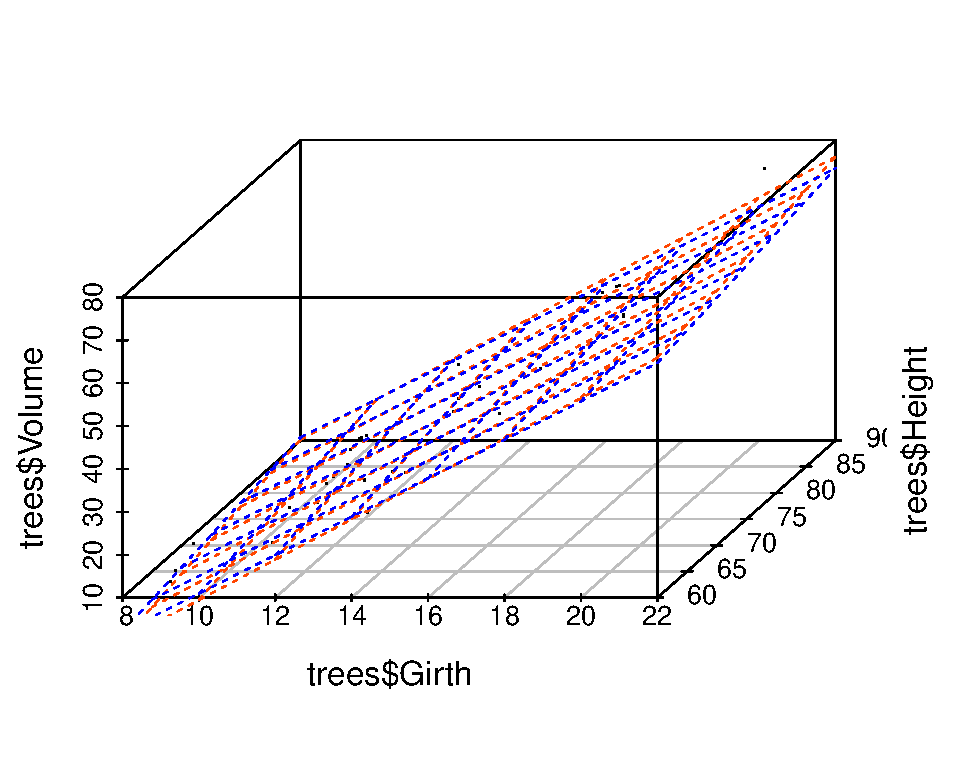
\includegraphics[width=0.5\columnwidth]{./figures/hands-on4/trees-jitterfit-volume.pdf}
\caption{Multiple regression plot of cherry tree volume on girth and height, for the original data (red) and the jittered data (blue).\label{fig:jittervolume}}
\end{figure}

Finally, let's do some vector calculations to quantify how the angular deviation between the fit data and the predictor variables changes between the original and jittered data set for the two different multiple regressions:
%
\begin{R}

# write a quickie fxn to express angle between vectors in degrees
> vec.angle <- function(x,y) { acos(cor(x,y)) * (180/pi)}

# vector angles for fit of Height ~ Girth + Volume (orig)
> vec.angle(lm.H$fitted.values, trees$Girth)
[1] 36.02644
> vec.angle(lm.H$fitted.values, trees$Volume)
[1] 21.29297

# vector angles for fit of Height ~ Girth + Volume (jittered)
> vec.angle(lm.H.jitter$fitted.values, jitter.trees$Girth)
[1] 28.48079
> vec.angle(lm.H.jitter$fitted.values, jitter.trees$Volume)
[1] 9.097828

# CONCLUSION -- angular changes of about 8 and 12 degrees 


# vector angles for fit of Volume ~ Girth + Height (orig)
> vec.angle(lm.V$fitted.values, trees$Girth)
[1] 6.628322
> vec.angle(lm.V$fitted.values, trees$Height)
[1] 52.08771

# vector angles for fit of Volume ~ Girth + Height (jittered)
> vec.angle(lm.V.jitter$fitted.values, jitter.trees$Girth)
[1] 6.163463
> vec.angle(lm.V.jitter$fitted.values, jitter.trees$Height)
[1] 54.33651

# CONCLUSION -- angular changes of about 0.5 and 2 degrees
\end{R}

\section{Manipulating data using split}

Last week we introduced the |reshape()| function from the reshape2 package.  |reshape()| is good for computing simple statistics across multiple `facets' of data. However, more complicated statistics are made possible by using the |split()| function, which is defined in the R base package.

|split()| takes two arguments: 1) a vector or data frame to split and 2) a character vector defining what to split the first argument by. For example, we can split the iris data set by species in order to get a list containing three data frames; one for each species.
%
\begin{R}
> iris.split <- split(iris, iris$Species)
> names(iris.split)
[1] "setosa"     "versicolor" "virginica" 
> str(iris.split)  # see the documentation for the str() function
List of 3
 $ setosa    :'data.frame': 50 obs. of  5 variables:
  ..$ Sepal.Length: num [1:50] 5.1 4.9 4.7 4.6 5 5.4 4.6 5 4.4 4.9 ...
  ..$ Sepal.Width : num [1:50] 3.5 3 3.2 3.1 3.6 3.9 3.4 3.4 2.9 3.1 ...
  ..$ Petal.Length: num [1:50] 1.4 1.4 1.3 1.5 1.4 1.7 1.4 1.5 1.4 1.5 ...
  ..$ Petal.Width : num [1:50] 0.2 0.2 0.2 0.2 0.2 0.4 0.3 0.2 0.2 0.1 ...
  ..$ Species     : Factor w/ 3 levels "setosa","versicolor",..: 1 1 1 1 1 1 1 1 1 1 ...
 $ versicolor:'data.frame': 50 obs. of  5 variables:
  ..$ Sepal.Length: num [1:50] 7 6.4 6.9 5.5 6.5 5.7 6.3 4.9 6.6 5.2 ...
  ..$ Sepal.Width : num [1:50] 3.2 3.2 3.1 2.3 2.8 2.8 3.3 2.4 2.9 2.7 ...
  ..$ Petal.Length: num [1:50] 4.7 4.5 4.9 4 4.6 4.5 4.7 3.3 4.6 3.9 ...
  ..$ Petal.Width : num [1:50] 1.4 1.5 1.5 1.3 1.5 1.3 1.6 1 1.3 1.4 ...
  ..$ Species     : Factor w/ 3 levels "setosa","versicolor",..: 2 2 2 2 2 2 2 2 2 2 ...
 $ virginica :'data.frame': 50 obs. of  5 variables:
  ..$ Sepal.Length: num [1:50] 6.3 5.8 7.1 6.3 6.5 7.6 4.9 7.3 6.7 7.2 ...
  ..$ Sepal.Width : num [1:50] 3.3 2.7 3 2.9 3 3 2.5 2.9 2.5 3.6 ...
  ..$ Petal.Length: num [1:50] 6 5.1 5.9 5.6 5.8 6.6 4.5 6.3 5.8 6.1 ...
  ..$ Petal.Width : num [1:50] 2.5 1.9 2.1 1.8 2.2 2.1 1.7 1.8 1.8 2.5 ...
  ..$ Species     : Factor w/ 3 levels "setosa","versicolor",..: 3 3 3 3 3 3 3 3 3 3 ...
\end{R}

Now that we have a split data frame, it's easy to use |lapply| or |sapply| to calculate complicated summary statistics. For example, this function calculates the mean ratio of |Sepal.Length| to |Petal.Length|:
%
\begin{R}
> ratio.sepal2petal <- function(x) {
+    mean( x$Sepal.Length / x$Petal.Length)
+ }
> sapply(iris.split, ratio.sepal2petal)
    setosa versicolor  virginica 
  3.464906   1.400896   1.188350 
\end{R}
%
We could also write a function to return the coefficients of fitting a linear model to each facet of the data:
%
\begin{R}
> sepal.on.petal.coeff <- function(x){
+       model <- lm(Sepal.Length ~ Petal.Length, data=x)
+       return(model$coeff)
+ }
> sapply(iris.split, sepal.on.petal.coeff)
                setosa versicolor virginica
(Intercept)  4.2131682   2.407523 1.0596591
Petal.Length 0.5422926   0.828281 0.9957386
\end{R}
%
Of course, no analysis would be complete without examining the fit of the linear models. In order to visualize whether the linear model is a good representation of the data, we'll write another function to return a data frame containing the fitted values, residuals, and species names for each element of the list.
%
\begin{R}
> sepal.on.petal.lm.fit <- function(x){
+       model <- lm(Sepal.Length ~ Petal.Length, data=x)
+       data.frame(fitted = fitted(model),
+                  residuals = residuals(model),
+                  species = x$Species)
+ }
> iris.fit <- lapply(iris.split, sepal.on.petal.lm.fit)
> str(iris.fit)
List of 3
 $ setosa    :'data.frame': 50 obs. of  3 variables:
  ..$ fitted   : num [1:50] 4.97 4.97 4.92 5.03 4.97 ...
  ..$ residuals: num [1:50] 0.1276 -0.0724 -0.2181 -0.4266 0.0276 ...
  ..$ species  : Factor w/ 3 levels "setosa","versicolor",..: 1 1 1 1 1 1 1 1 1 1 ...
 $ versicolor:'data.frame': 50 obs. of  3 variables:
  ..$ fitted   : num [1:50] 6.3 6.13 6.47 5.72 6.22 ...
  ..$ residuals: num [1:50] 0.7 0.265 0.434 -0.221 0.282 ...
  ..$ species  : Factor w/ 3 levels "setosa","versicolor",..: 2 2 2 2 2 2 2 2 2 2 ...
 $ virginica :'data.frame': 50 obs. of  3 variables:
  ..$ fitted   : num [1:50] 7.03 6.14 6.93 6.64 6.83 ...
  ..$ residuals: num [1:50] -0.734 -0.338 0.165 -0.336 -0.335 ...
  ..$ species  : Factor w/ 3 levels "setosa","versicolor",..: 3 3 3 3 3 3 3 3 3 3 ...
> 
\end{R}

Next, we'll join the data back into a data frame using the |do.call| and |rbind| functions. Read the documentation to figure out what they do.
%
\begin{R}
> iris.joined <- do.call('rbind', iris.fit)
> str(iris.joined)
'data.frame': 150 obs. of  3 variables:
 $ fitted   : num  4.97 4.97 4.92 5.03 4.97 ...
 $ residuals: num  0.1276 -0.0724 -0.2181 -0.4266 0.0276 ...
 $ species  : Factor w/ 3 levels "setosa","versicolor",..: 1 1 1 1 1 1 1 1 1 1 ...
\end{R}

Finally, we'll visualize our model fits by plotting our data using ggplot:
%
\begin{R}
> library(ggplot2)
> ggplot(iris.joined, aes(x=fitted, y=residuals))+
+   geom_point()+
+   facet_wrap(~species, scale='free') + 
+   ggtitle("Residuals from Regression of \nSepal Length on Petal Length for 3 Iris Species")
\end{R}
Examining the residuals (Fig.~\ref{fig:irissplit}), we see they look fairly uniform across the range of fit values. The term that statiscians use for this is `homoscedastic'; when the residuals are non uniform we say they are `heteroscadistic'.
%
\begin{figure}[htbp]
\centering
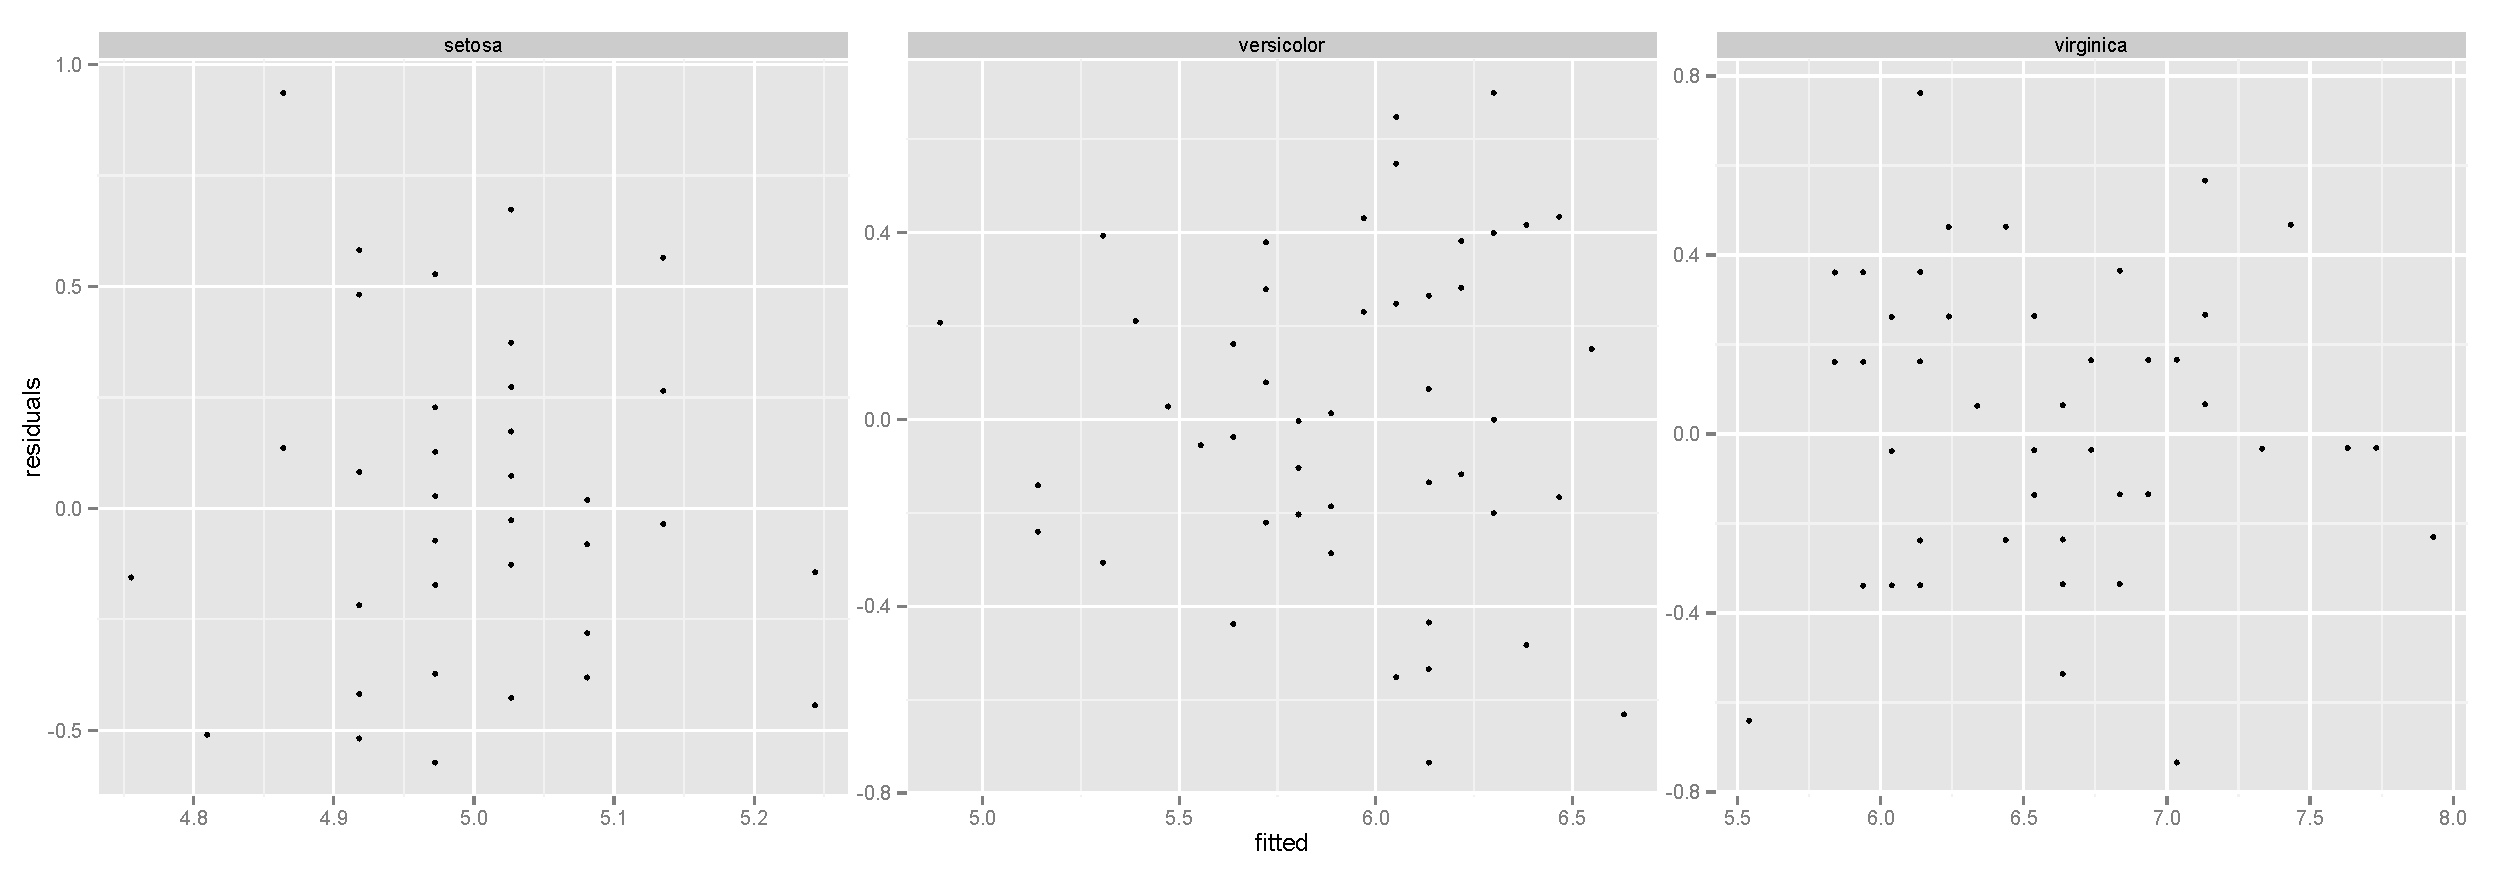
\includegraphics[width=0.75\columnwidth]{./figures/hands-on4/iris-residuals.pdf}
\caption{Residuals from regressions of Sepal Length on Petal Length, for the Iris data set split by species.\label{fig:irissplit}}
\end{figure}


An alternate way to visualize the fits, without the benefit of  getting the info on the model fits back for further examination, is to use the |stat_smooth()| to plot a linear fit of our data for each facet (Fig.~\ref{fig:irisregressions}). Read the |stat_smooth| documentation to how this works.
%
\begin{R}
> ggplot( iris, aes(x=Petal.Length, y=Sepal.Length))+
   geom_point()+
   stat_smooth(method="lm")+
   facet_wrap(~Species, scale='free')+
   ggtitle("Regressions of Sepal Length on Petal Length")
\end{R}
%
\begin{figure}[htbp]
\centering
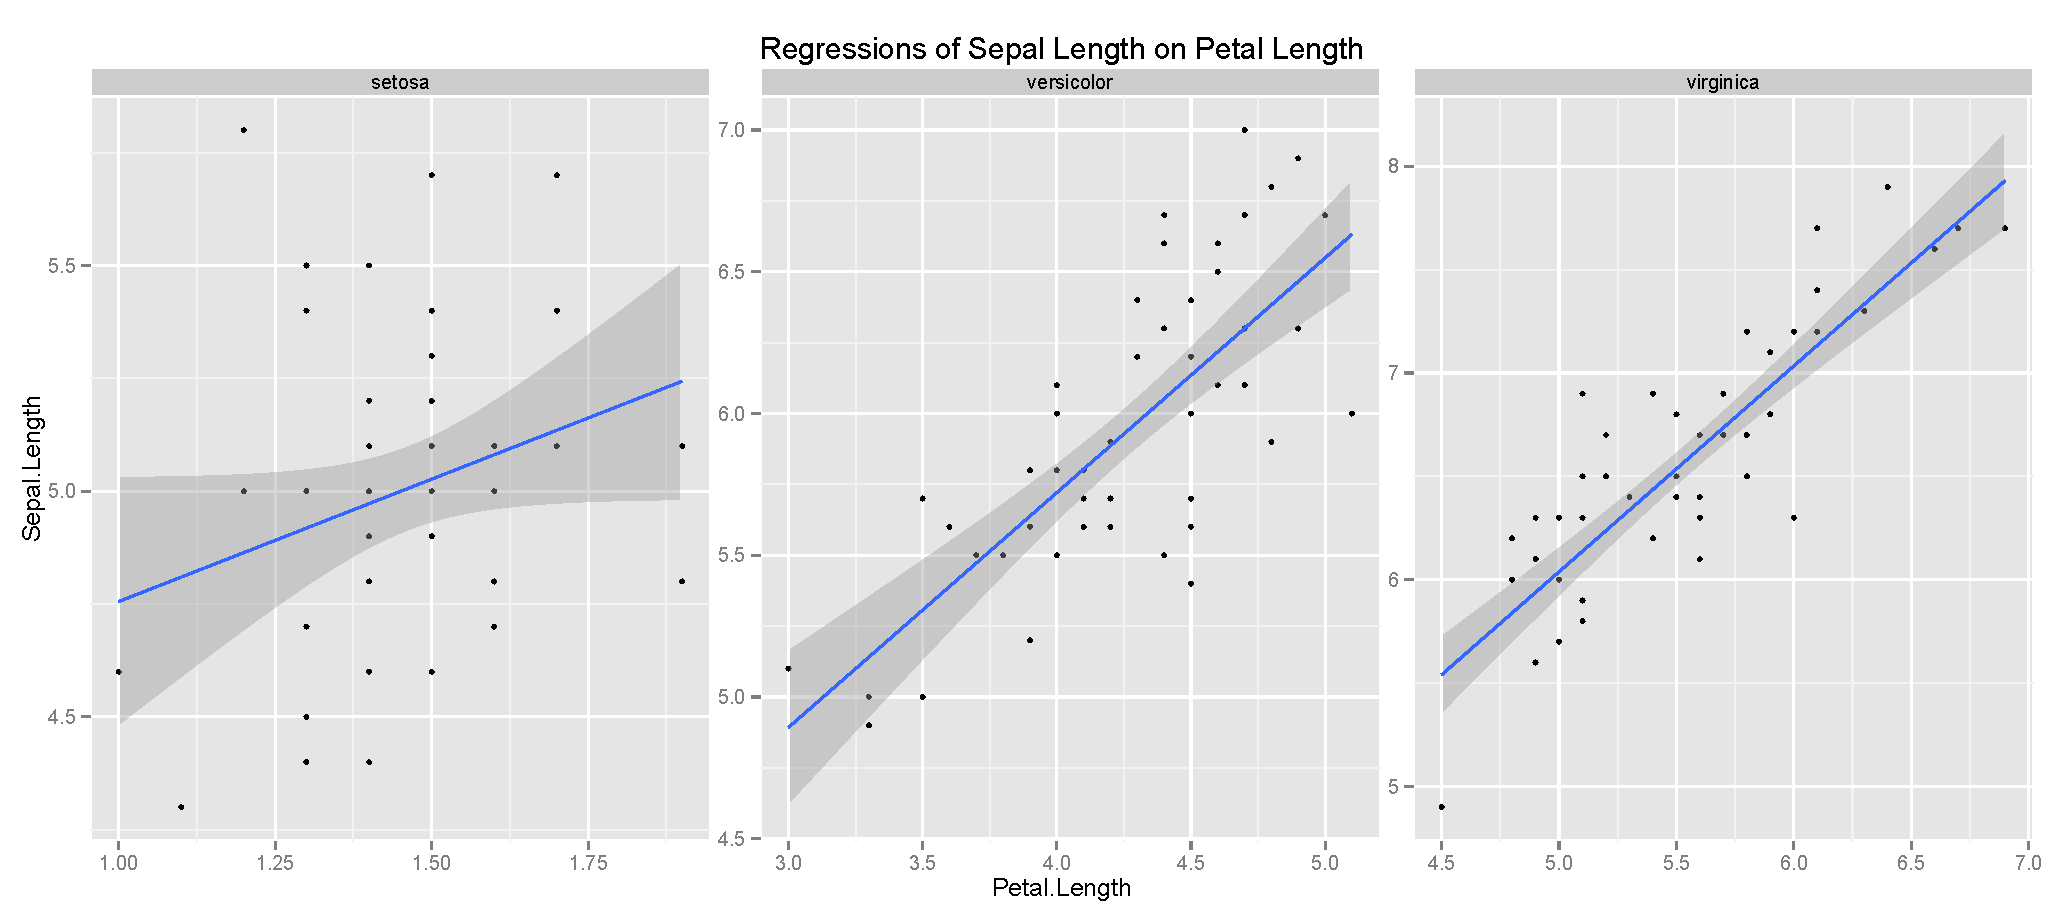
\includegraphics[width=0.75\columnwidth]{./figures/hands-on4/iris-regressions.pdf}
\caption{Regressions of Sepal Length on Petal Length, for the Iris data, produced using the \lstinline|stat_smooth()| function in ggplot2.\label{fig:irisregressions}}
\end{figure}
%
